%%%%%%%%%%%%%%%%%%%%%%%%%%%%%%%%%%%%%%%%%%%%%%%%%%%%%%%%%%%%
%\documentclass[xcolor=x11names,compress]{beamer}
\documentclass[handout]{beamer}
\definecolor{CoolBlack}{rgb}{0.0, 0.18, 0.39}
\definecolor{byellow}{rgb}{0.55037, 0.38821, 0.06142}
%% General document %%%%%%%%%%%%%%%%%%%%%%%%%%%%%%%%%%
\usepackage{graphicx}
\usepackage{tikz}
\usepackage{Tabbing, tabu}
\usetikzlibrary{decorations.fractals}
%%%%%%%%%%%%%%%%%%%%%%%%%%%%%%%%%%%%%%%%%%%%%%%%%%%%%%

%% Beamer Layout %%%%%%%%%%%%%%%%%%%%%%%%%%%%%%%%%%
\useoutertheme[subsection=false,shadow]{miniframes}
\useinnertheme{default}
\usefonttheme{serif}
\usepackage{palatino}
\usepackage{tabu}

% addition of color
\usepackage{xcolor}
\definecolor{dgreen}{rgb}{0.,0.6,0.}
\definecolor{RawSienna}{cmyk}{0,0.72,1,0.45}

\setbeamerfont{title like}{shape=\scshape}
\setbeamerfont{frametitle}{shape=\scshape}

\setbeamercolor*{lower separation line head}{bg=CoolBlack} 
\setbeamercolor*{normal text}{fg=black,bg=white} 
\setbeamercolor*{alerted text}{fg=dgreen} 
\setbeamercolor*{example text}{fg=black} 
\setbeamercolor*{structure}{fg=black} 
 
\setbeamercolor*{palette tertiary}{fg=black,bg=black!10} 
\setbeamercolor*{palette quaternary}{fg=black,bg=black!10} 

% Links
\usepackage{hyperref}
\definecolor{links}{HTML}{003262}
\hypersetup{colorlinks,linkcolor=,urlcolor=links}

% columns
\renewcommand{\(}{\begin{columns}}
\renewcommand{\)}{\end{columns}}
\newcommand{\<}[1]{\begin{column}{#1}}
\renewcommand{\>}{\end{column}}

% adding slide numbers
\addtobeamertemplate{navigation symbols}{}{%
    \usebeamerfont{footline}%
    \usebeamercolor[fg]{footline}%
    \hspace{1em}%
    \insertframenumber/\inserttotalframenumber
}

% equation stuff
\newcommand{\Macro}{\ensuremath{\Sigma}}
\newcommand{\Sn}{\ensuremath{S_N} }
\newcommand{\vOmega}{\ensuremath{\hat{\Omega}}}
\usepackage{mathrsfs}
\usepackage[mathcal]{euscript}
\usepackage{amssymb}
\usepackage{amsthm}
\usepackage{epsfig}
\usepackage{amsmath}

\newcommand{\ve}[1]{\ensuremath{\vec{#1}}}
\newcommand{\micro}{\ensuremath{\sigma}}
\newcommand{\detR}{\ensuremath{\Sigma}}

\newcommand{\vecr}{\vec{r}}
\newcommand{\sn}{S$_\mathrm{N}$~}
\newcommand{\pn}{P$_\mathrm{N}$~}
\newcommand{\sigt}{\Sigma_t}
\newcommand{\sigs}{\Sigma_s}
\newcommand{\hn}{\mathcal{H}_N}
\newcommand{\maths}{\mathbb{S}^2}
\newcommand{\dn}{d_N}
\newcommand{\lij}{\langle L_i,L_j \rangle}

\newcommand{\Jij}[2]{\ensuremath{\int L(\vOmega_#1)L(\vOmega_#2)}}
\newcommand{\Gij}[2]{\ensuremath{\sum_{\ell=0}^L \frac{2\ell +1}{4\pi}P_{\ell}(\vOmega_#1 \cdot\vOmega_#2)}}
\newcommand{\LijJij}[4]{\ensuremath{\int L_#1(\vOmega_#3)L_#2(\vOmega_#4)}}
\newcommand{\Sij}[2]{\ensuremath{\Sigma^{g'\rightarrow g}_{\text{s,N}}(\vOmega_#1 \cdot \vOmega_#2)}}

\newcommand{\sigg}[1]{\ensuremath{\sigma^{gg'}_{\text{s}\,#1}}}
\newcommand{\Sigg}[1]{\ensuremath{\Sigma^{gg'}_{\text{s}\,#1}}}
\newcommand{\psig}{\ensuremath{\psi^g}}
\newcommand{\ldosig}[2]{\ensuremath{\sum_{n=0}^N \frac{2n+1}{4\pi}\sigma_{s,n}^{g'\rightarrow g} P_n(\vOmega_#1\cdot\vOmega_#2)}}


\newcommand\RBox[1]{%
  \tikz\node[draw,rounded corners,align=center,] {#1};}%

\setbeamerfont{author in head/foot}{size={\fontsize{3pt}{4pt}\selectfont}}
%\author[Subham \& Mithun \& Karthikeyan \& Shantikumar]
%{%
%   \texorpdfstring{
%        \begin{columns}
%            \column{.25\linewidth}
%            \centering
%            \includegraphics[height=3cm]{../bk-eps-converted-to}
%            \column{.25\linewidth}
%            \centering
%            \RBox{R.\ N.\ Slaybaugh\\
%            Univ.\ of Cal.\ Berkeley}\\[1ex]
%            \RBox{T.\ M.\ Evans, and\\
%            S.\ W.\ Mosher\\
%            Oak Ridge National Lab}
%        \end{columns}
%   }
%   {Subham Soni S., Karthikeyanm, Shantikumar L.,  Mithun C.K.}
%}
\title{Improved Hybrid Modeling}
\subtitle{of Used Fuel Storage Facilities}
\author{\includegraphics[height=2cm]
{../bk-eps-converted-to}\\R.\ N.\ Slaybaugh, Univ.\ of Cal.\ Berkeley\\[1ex]
T.\ M.\ Evans and S.\ W.\ Mosher, Oak Ridge National Lab}
\date{30 March 2017 \\ DOE MPACT Meeting, Albuquerque, NM}

%%%%%%%%%%%%%%%%%%%%%%%%%%%%%%%%%%%%%%%%%%%%%%%%%%

\begin{document}

%%%%%%%%%%%%%%%%%%%%%%%%%%%%%%%%%%%%%%%%%%%%%%%%%%%%%%
%%%%%%%%%%%%%%%%%%%%%%%%%%%%%%%%%%%%%%%%%%%%%%%%%%%%%%
\begin{frame}
\titlepage
\end{frame}

% --------------------------------------------------------------
\begin{frame}[fragile]{Outline}
  \frametitle{Outline}

\begin{columns}
  \begin{column}{0.5\textwidth}
    \begin{itemize}
    \item Motivation
    \vspace*{.75em}
    \item Hybrid Methods and Strong Anisotropies
    \vspace*{.75em}
	\item CADIS-$\Omega$ Method
    \vspace*{.75em}
	\item Results and Plans
    \vspace*{.75em}
	\item LDO Method
  \end{itemize}
  \end{column}
  \begin{column}{0.5\textwidth}
  	\begin{figure}
  	\begin{center}
  		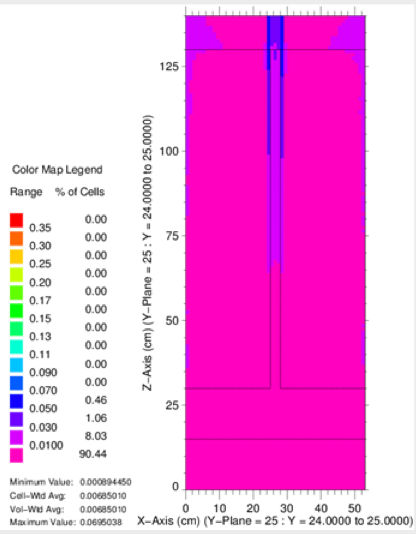
\includegraphics[height=2.5in,clip]{plate-air}
		\caption{relative error; steel plate in moderator \cite{Wilson2015}}
		%For particles near the turns in the labyrinth, the importance of the particles to the exit of the labyrinth vary greatly if they are coming out of a wall pointed toward the exit versus heading into a wall and away from the exit. This distinction is not captured by current hybrid methods. 
	\end{center}
  	\end{figure}
  \end{column}
\end{columns}

\end{frame}


% --------------------------------------------------------------
% --------------------------------------------------------------
\section{\scshape Motivation \& Background}
\begin{frame}[fragile]
  \frametitle{Project motivation}

\begin{columns}
  \begin{column}{0.55\textwidth}
	\begin{itemize}
	\item Need to accurately model radiation for safeguarding and monitoring
	\item \alert{Challenging}: dense shields; streaming paths
	\item Current methods are insufficient
	\item \alert{Goal}: accurate solutions in reasonable time
	\item New methods can easily be added to existing codes
	\end{itemize}
  \end{column}
  \begin{column}{0.45\textwidth}
  	\begin{figure}
  	\begin{center}
  		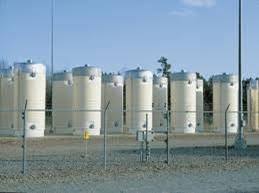
\includegraphics[height=1.5in,clip]{../figs/isfsi}
		\caption{Used fuel storage pad}
	\end{center}
  	\end{figure}
  \end{column}
\end{columns}

\end{frame}

% --------------------------------------------------------------
% --------------------------------------------------------------
\begin{frame}[fragile]
  \frametitle{Solving the TE}
%
\begin{columns}
  \begin{column}{0.5\textwidth}
  \begin{center}
  \underline{Monte Carlo}
  \end{center}
	\begin{itemize}
	\item Solution has statistical error
	\item \textit{Continuous} phase space%: ``gold standard answers"
	\item Can be slow
	\item Optically thick = \textit{slow}
	\end{itemize}
  \end{column}
  \begin{column}{0.5\textwidth}
  \begin{center}
  \underline{Deterministic}
  \end{center}
	\begin{itemize}
	\item Solution equally valid everywhere
	\item \textit{Discretized} phase space%: drives solution quality
	\item Can be fast
	\item Streaming = \textit{ray effects}
	\end{itemize}
  \end{column}
\end{columns}
%
\begin{align}
\vOmega \cdot \nabla \psi(\vec{r}, E, \vOmega) &+
\Sigma_t \psi(\vec{r}, E, \vOmega) = S(\vec{r}, E, \vOmega) \:+\nonumber\\
%
& \int_{4\pi} d\vOmega' \int_0^{\infty} dE'\: \Sigma_s(E', \vOmega' \rightarrow E, \vOmega) \psi(\vec{r}, E', \vOmega') \nonumber
\end{align}

\end{frame}

% --------------------------------------------------------------
\begin{frame}[fragile]
  \frametitle{Speeding up MC}
  \begin{itemize}
	\item Variance reduction (VR) used to improve Monte Carlo:\\
	reduce relative error \textit{and} time by augmenting game
	\item Particles are assigned weights that map to impact
	\item VR can be used to
	  \begin{itemize}
	  \item set weights at birth
	  \item update weights throughout problem
      \end{itemize}
      \pause
  \item Improvement measured as    
  \end{itemize}
\[
\text{FOM} = \frac{1}{\text{R}^2\text{t}} \quad \text{R = relative error;  t = time} 
\]
\pause
\textbf{Hybrid Methods:} we use deterministic results to make Monte Carlo VR parameters

\end{frame}


% --------------------------------------------------------------
% --------------------------------------------------------------
%\section{\scshape Strong Anisotropies}
\begin{frame}[fragile]
  \frametitle{Anisotropy: a computational challenge}

	\begin{columns}
  	\begin{column}{0.5\textwidth}
	\begin{itemize}
	\item Many important nuclear applications have strong anisotropies
	 \begin{itemize}
	 \item \textbf{Used fuel casks}
	 \item Reprocessing facilities
	 \item Reactor facilities
	 \item Active interrogation 
	 \end{itemize}
	\pause
	\item New ideas are needed for these problems
	\begin{itemize}
	\item Current hybrid methods are insufficient
	\item Including angle explicitly is too costly	
	\end{itemize}
	\end{itemize}
  	\end{column}
 	%
 	\begin{column}{0.5\textwidth}
 	 \begin{center}
 	 \begin{figure}
 	 \includegraphics[height=2in,clip]{../figs/pwr}  
 	 \caption{PWR relative error \cite{Pantelias2013}}
 	 \end{figure}
 	 \end{center}

  	\end{column}
	\end{columns}

\end{frame}


% --------------------------------------------------------------
\begin{frame}[fragile]
  \frametitle{Forward-Adjoint Relationship \cite{Wagner2007}}
Define response with function $f(\ve{r}, E)$ in volume $V_f$ as
%
\begin{equation}
 R = \int_E \int_{V_f} f(\ve{r}, E) \phi(\ve{r}, E) dV dE 
 \label{eq:Response}
\end{equation}
%
\begin{columns}
  \begin{column}{0.5\textwidth}
	\begin{align}
  	H\phi &= q \quad \text{(forward)}\nonumber \\
  	%
  	H^{\dagger} \phi^{\dagger} &= q^{\dagger} \quad 
  	\text{(adjoint)}\nonumber
  	\end{align}
  \end{column}
  \begin{column}{0.5\textwidth}
  	\begin{align}
  	\langle H\phi, \phi^{\dagger} \rangle &= \langle H^{\dagger} \phi^{\dagger}, \phi \rangle \:, \text{and therefore} \nonumber \\
  	%
  	\langle q, \phi^{\dagger} \rangle &= \langle q^{\dagger}, \phi \rangle \nonumber
  	\end{align}
  \end{column}
\end{columns}
\vspace*{1 em}
If we let $q^{\dagger} = f(\ve{r}, E)$ then
%
\begin{equation}
 \langle q^{\dagger}, \phi \rangle = \langle f, \phi \rangle = R = \langle q, \phi^{\dagger} \rangle
 \label{eq:ResponseRedef}
\end{equation}
%
Eq.\ \eqref{eq:ResponseRedef} expresses that $\phi^{\dagger}$ represents the expected contribution of a source particle to the response given the source, $q$.

\end{frame}

% --------------------------------------------------------------
\begin{frame}[fragile]
  \frametitle{CADIS \cite{Wagner2007}}
  
  \begin{enumerate}
  \item Define $q^{\dagger}$ as the local response of interest\\
  \item Coarse deterministic calculation to get $\phi^{\dagger}$ and $R$
  \end{enumerate}
% 
\begin{align}
  imp(\ve{r}, E) &= \frac{\phi^{\dagger}(\ve{r}, E)}{\langle q(\ve{r}, E), \phi^{\dagger}(\ve{r}, E) \rangle} = \frac{\phi^{\dagger}(\ve{r}, E)}{R} \\
  %
  \hat{q}(\ve{r}, E) &= \frac{\phi^{\dagger}(\ve{r}, E) q(\ve{r}, E)}{R} \\
  %
  w_0(\ve{r}, E) &= \frac{q(\ve{r}, E)}{\hat{q}(\ve{r}, E)} = \frac{R}{\phi^{\dagger}(\ve{r}, E)} 
  \label{eq:Importance}
\end{align}

Birth weights match weight targets, making this the \underline{C}onsistent \underline{A}djoint \underline{D}riven \underline{I}mportance \underline{S}ampling \underline{M}ethod

\end{frame}

% --------------------------------------------------------------
%\subsection{FW-CADIS}
\begin{frame}[fragile]
  \frametitle{FW-CADIS \cite{Wagner2007}}

\begin{itemize}
\item We often what to optimize solutions in all of phase space\\
\item In this case the adjoint source needs to be a global forward solution: \underline{F}orward \underline{W}eighted-CADIS
\end{itemize}
%
\begin{columns}
  \begin{column}{0.5\textwidth}
  \begin{center}
  \alert{To Optimize}
  \end{center}
	\begin{align}
  	&\phi(\ve{r}, E)\nonumber \\
  	%
  	\int&\phi(\ve{r}, E)\sigma_d(\ve{r}, E)\nonumber
  	\end{align}
  \end{column}
  %
  \begin{column}{0.5\textwidth}
  \begin{center}
  \alert{Adjoint Source}
  \end{center}
  	\begin{align}
  	f(\ve{r}, E) &= \frac{1}{\phi(\ve{r}, E)}\nonumber \\
  	%
  	f(\ve{r}, E) &= \frac{\sigma_d(\ve{r}, E)}{\int\phi(\ve{r}, E)\sigma_d(\ve{r}, E)} \nonumber
  	\end{align}
  \end{column}
\end{columns}
\vspace*{1 em}
For example
%
\begin{equation}
 R = \int_E \int_{V_f} f(\ve{r}, E) \phi(\ve{r}, E) dV dE = \int_E \int_{V} \frac{1}{\phi(\ve{r}, E)} \phi(\ve{r}, E) dV dE \approx 1 \nonumber
\end{equation}

\end{frame}


% --------------------------------------------------------------
%\begin{frame}[fragile]
%  \frametitle{Adjoint as an importance map}
%Use \textit{adjoint}: the importance of a source particle to the solution
%
%\begin{itemize}
%\item Forward ($\phi$ or $\psi$): neutrons flow from the source to the detector
%\item Adjoint($\phi^{\dagger}$ or $\psi^{\dagger}$): particles represent how each part of phase space contributes to the ``source"
%\item The current state of the art is FW/CADIS \cite{Wagner2007}
%\end{itemize}
%\begin{align*}
%  imp(\ve{r}, E) &= \frac{\phi^{\dagger}(\ve{r}, E)}{\langle q(\ve{r}, E), \phi^{\dagger}(\ve{r}, E) \rangle} = \frac{\phi^{\dagger}(\ve{r}, E)}{R} \\
%  %
%  \hat{q}(\ve{r}, E) &= \frac{\phi^{\dagger}(\ve{r}, E) q(\ve{r}, E)}{R} \\
%  %
%  w_0(\ve{r}, E) &= \frac{q(\ve{r}, E)}{\hat{q}(\ve{r}, E)} = \frac{R}{\phi^{\dagger}(\ve{r}, E)} 
%\end{align*}
%
%\end{frame}


% --------------------------------------------------------------
\begin{frame}[fragile]
  \frametitle{Current hybrid methods are insufficient}

\[\text{Note:}\qquad\phi^{\dagger}(\ve{r},E) = \int \psi^{\dagger}(\vOmega, 
		\ve{r},E) d\vOmega\]

	\begin{itemize}
	\item MC VR parameters created from adjoint deterministic scalar flux that is a function of \textit{space and energy only} \vspace*{1 em}
	\pause
	\item Angular dependence of the importance function is not retained, otherwise the map would be 
	\begin{itemize}
	  \item very large (tens or hundreds of GB) and
	  \item more costly and complex to use in the MC simulation 
	\end{itemize}
	\pause
	\item Drawback: within a given space/energy cell, map provides average importance of a particle moving in \textit{any direction} through the cell--excluding information about how particles move \alert{toward the objective}
	\end{itemize}

\end{frame}

% --------------------------------------------------------------
\begin{frame}[fragile]
  \frametitle{Current hybrid methods are insufficient}

	\begin{columns}
  	\begin{column}{0.5\textwidth}
 	 \begin{center}
 	 \begin{figure}
 	 \includegraphics[height=2in,clip]{../figs/boat-interrogation}  
 	 \caption{Spherical boat model with source on left and fissionable material at center}
 	 \end{figure}
 	 \end{center}
  	\end{column}
 	%
 	\begin{column}{0.5\textwidth}
 	 \begin{center}
 	 \begin{figure}
 	 \includegraphics[height=2in,clip]{../figs/boat-map}  
 	 \caption{Target weight window values for 14.1 MeV neutrons}
 	 \end{figure}
 	 \end{center}
  	\end{column}
	\end{columns}

\end{frame}

% --------------------------------------------------------------
% --------------------------------------------------------------
% --------------------------------------------------------------
\section{\scshape CADIS-$\Omega$}
\begin{frame}[fragile]
  \frametitle{Integration weighting}

    Different integration plan captures angles in scalar flux creation	
	\begin{align*}
		\phi^{\dagger}(\ve{r},E) &= \int \psi^{\dagger}(\vOmega, 
		\ve{r},E) d\vOmega \qquad  \qquad \qquad \text{original}\\
		 %
		\phi^{\dagger}(\ve{r},E) &= \frac{\int \psi(\vOmega, \ve{r},E)
		 \psi^{\dagger}(\vOmega, \ve{r},E) d\vOmega}{\int \psi(\vOmega, 
		 \ve{r},E)  d\vOmega} \qquad \text{\alert{new}}
	\end{align*}
%Note that these two calculations can be completed concurrently. Then, the adjoint scalar fluxes will be computed by angularly integrating the product of the forward and adjoint angular fluxes to account for the directions in which the particles will actually be traveling at any given location/energy:
%will provide importance values that more accurately reflect the average importance of particles that will be transported in the final Monte Carlo calculation, yielding faster Monte Carlo run times.
    \pause
    Major challenges and areas of investigation:
	\begin{enumerate}
	\item Data storage and handling (many GBs)
	\item More, less, or differently sensitive to 
	  \begin{itemize}
	  \item quality of the discrete ordinates calculation?
	  \item ray effects?
	  \end{itemize}
	\end{enumerate}

\end{frame}


% --------------------------------------------------------------
\begin{frame}[fragile]
  \frametitle{Method implementation}

  	\begin{itemize}
    \item The space- and energy-dependent importance map is normalized and 
     source biasing parameters are generated in the \alert{same ways} as
     the current implementation of FW/CADIS \vspace*{1 em}
	\item Immediately useful; widely applicable \vspace*{1 em}
	\item We are studying and characterizing the impact\vspace*{1 em}
	\item Is available ADVANTG \cite{mosher_new_2010}
	\end{itemize}
	
\end{frame}


% --------------------------------------------------------------
% --------------------------------------------------------------
\section{\scshape Results \& Plans}
\begin{frame}[fragile]
  \frametitle{Current Status}

    \begin{enumerate}
    \item Implementation: \alert{complete}
      \begin{itemize}
      %\item Large data handling is \alert{broader outcome}
      \item Implementation of weighted flux algorithm in Denovo \cite{Evans2010} is 
      complete
      \item Integration of method into ADVANTG complete
      %\item ADVANTG allows for ease of use; broader user base
      %\item Denovo integration enhances use on other hybrid platforms
      \end{itemize} 
      \vspace*{0.5em}
      \pause
    \item Testing: \alert{in process}
      \begin{itemize}
      \item A collection of small tests with varying anisotropies
      \item Study performance compared to existing methods as a function of degree of anisotropy
      \item Investigate impact of angular discretization
      \end{itemize}
      \vspace*{0.5em}
      \pause
    \item Impact characterization: \alert{started}
      \begin{itemize}
      \item Investigate performance for one used fuel canister
      \item Investigate performance for array of used fuel canisters
      \item \alert{Goal}: improved material control and accountability
      \end{itemize}
    \end{enumerate}

	
\end{frame}

%% --------------------------------------------------------------
%% --------------------------------------------------------------
%%\section{\scshape Initial Results}
%\begin{frame}[fragile]
%
%  \frametitle{Results 1: maze problem}
%  10 MeV isotropic point source
%  \begin{columns}
%   \begin{column}{0.45\textwidth}
%   \begin{itemize}
%\item Concrete maze
%\item Air duct
%\end{itemize}
%   \end{column}
%  %
%  \begin{column}{0.5\textwidth}
%   \begin{itemize}
%\item NaI detector; 26 groups
%\item Reflecting BCs
%\end{itemize}
%   \end{column}
%\end{columns}
%   \begin{figure}
%   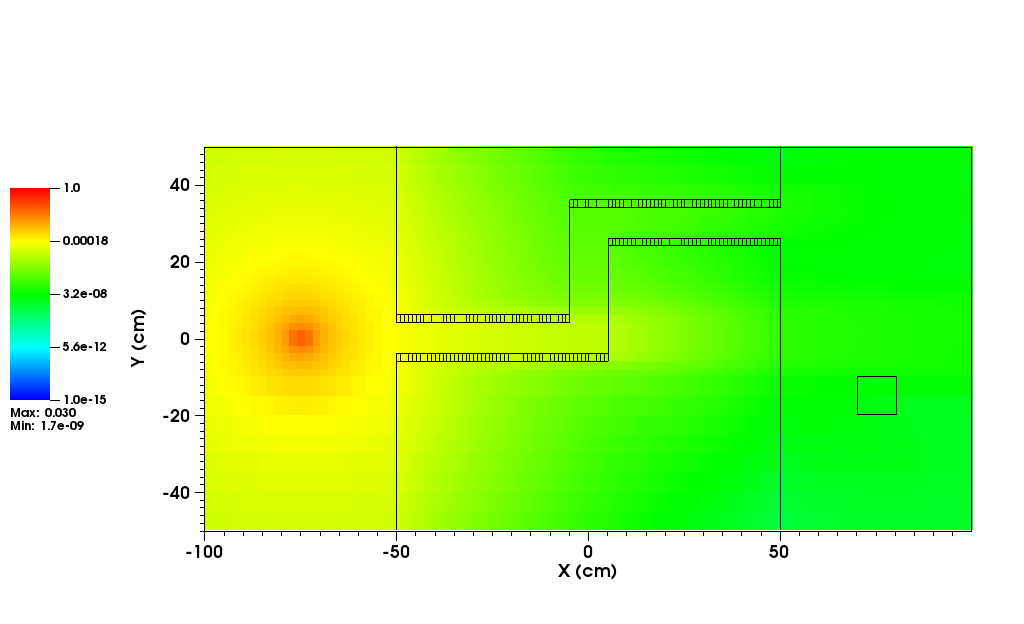
\includegraphics[height=2in,clip]{maze2_forward_group00_adjusted.png}
%   %\caption{Simple two-turn labyrinth}
%   \end{figure}
%
%
%	
%\end{frame}
%
%%% --------------------------------------------------------------
%%
%\begin{frame}[fragile]
%  \frametitle{Quantifying Anisotropy}
%  
%    \begin{columns}
%    \begin{column}{0.5\textwidth}
%  	\begin{figure}
%  	\begin{center}
%  		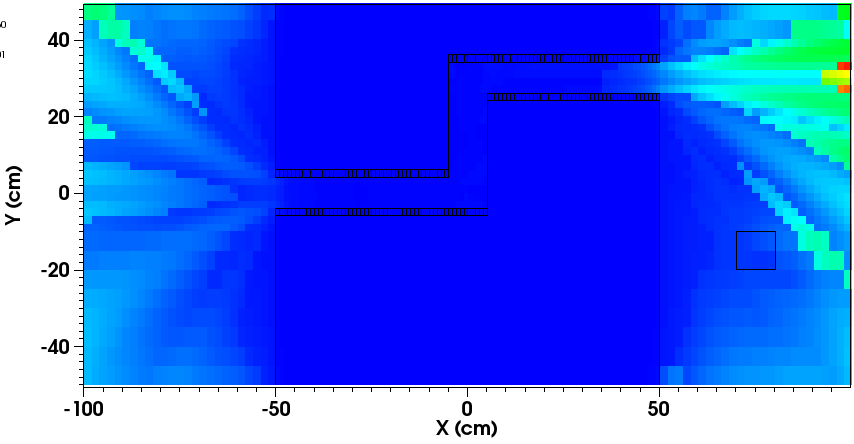
\includegraphics[height=1.1in,clip]{maze2_anisotropy_forward_group26_cropped.png}
%		%\caption{Forward flux anisotropy}
%	\end{center}
%  	\end{figure}
%  	  \begin{figure}
%  	\begin{center}
%  		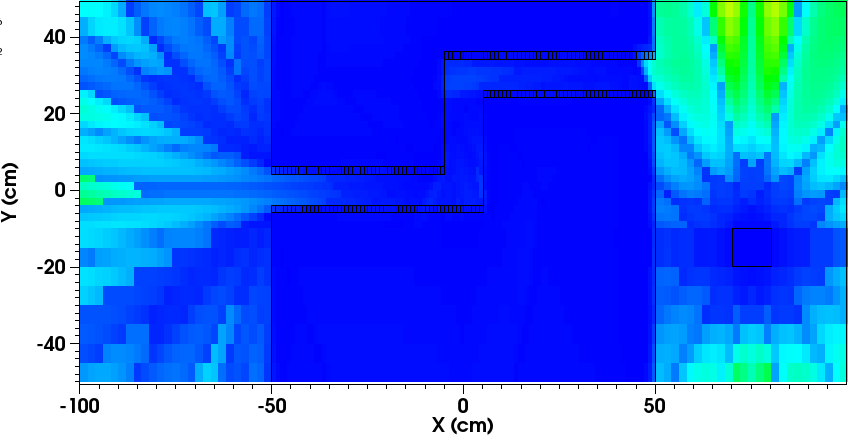
\includegraphics[height=1.1in,clip]{maze2_anisotropy_adjoint_group26_cropped.png}
%		%\caption{Adjoint flux anisotropy}
%	\end{center}
%  	\end{figure}
%    \end{column}
%  \pause
%    \begin{column}{0.5\textwidth}
%    Combining forward and adjoint fluxes, we see:
%    \begin{itemize}
%        \item Some elimination of ray effects
%        \item Anisotropy captured 
%    \end{itemize}
%  	\begin{figure}
%  	\begin{center}
%  		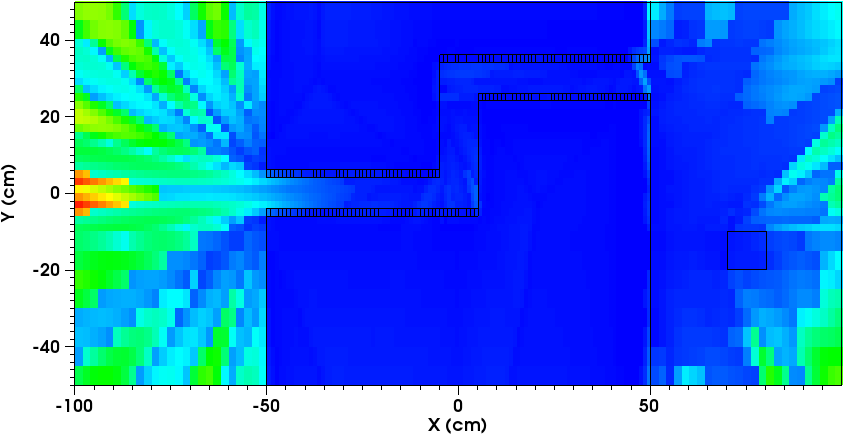
\includegraphics[height=1.1in,clip]{maze2_anisotropy_contributon_group26_cropped.png}
%		%\caption{Contributon flux anisotropy }
%	\end{center}
%  	\end{figure}
%  	\end{column}  
%  \end{columns}
%\end{frame}
%
%%% --------------------------------------------------------------
%
%\begin{frame}[fragile]
%  \frametitle{Generating adjusted fluxes}
%  %However, the method is not dominated by \textbf{just} the anisotropy....
%  \begin{columns}
%    \begin{column}{0.5\textwidth}
%  	\begin{figure}
%  	\begin{center}
%  		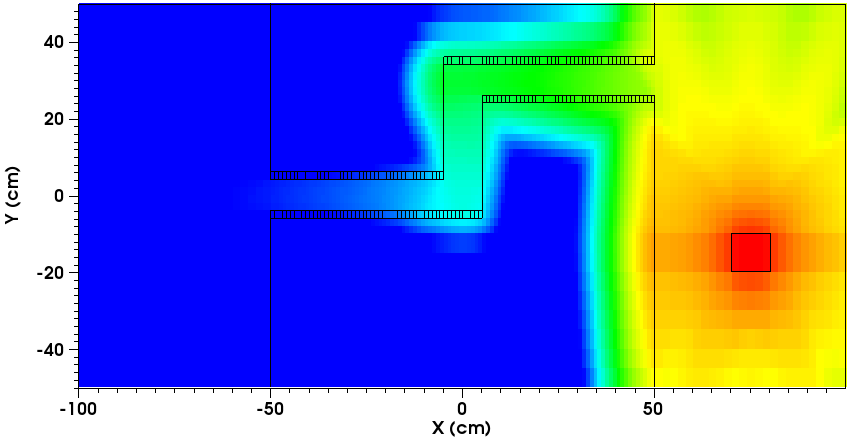
\includegraphics[height=1.1in,clip]{maze2_adjoint_group26_adjusted_cropped.png}
%		%\caption{Regions with high importance}
%	\end{center}
%  	\end{figure}
%  	  \begin{figure}
%  	\begin{center}
%  		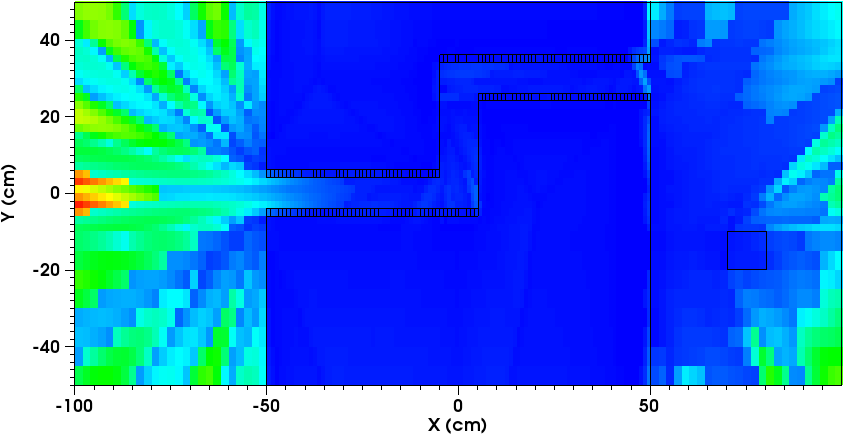
\includegraphics[height=1.1in,clip]{maze2_anisotropy_contributon_group26_cropped.png}
%		%\caption{... coupled with strong anisotropies}
%		% point out that while the FOM is better for analog, it has high RE in regions, so overall it performs poorer
%	\end{center}
%  	\end{figure}
%    \end{column}
%  \pause
%    \begin{column}{0.5\textwidth}
%   Regions with high importance coupled with strong anisotropy result in adjusted flux incorporating both
%  	\begin{figure}
%  	\begin{center}
%  		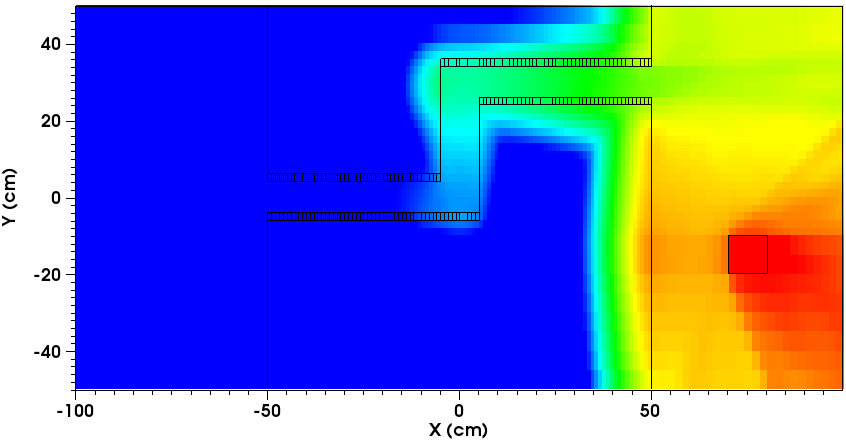
\includegraphics[height=1.1in,clip]{maze2_myflux_group26_adjusted_cropped.png}
%		%\caption{Result in adjusted flux incorporating both }
%	\end{center}
%  	\end{figure}
%  	\end{column}  
%  \end{columns}
%  %\alert{The new method incorporates both importance AND anisotropy into weighting parameters}
%\end{frame}
%
%%% --------------------------------------------------------------
%
%\begin{frame}[fragile]
%  \frametitle{Adjusted Fluxes}
%
%
%	Comparing the original adjoint to CADIS-$\Omega$....
%	\vspace*{1 em}
%	\begin{columns}
%  	\begin{column}{0.5\textwidth}
%  	\begin{figure}
%  	\begin{center}
%  		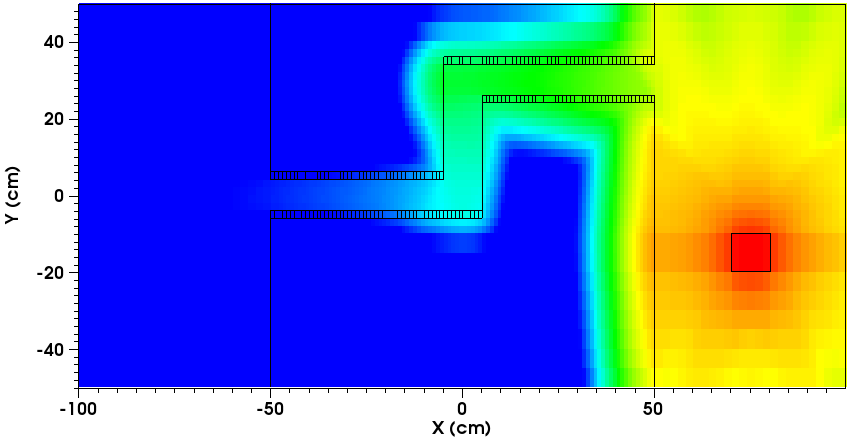
\includegraphics[height=1in,clip]{maze2_adjoint_group26_adjusted_cropped.png}
%		%\caption{Adjoint flux used by CADIS}
%	\end{center}
%  	\end{figure}
%  	\end{column}
% 	%
% 	\begin{column}{0.5\textwidth}
% 	\begin{figure}
%  	\begin{center}
%  		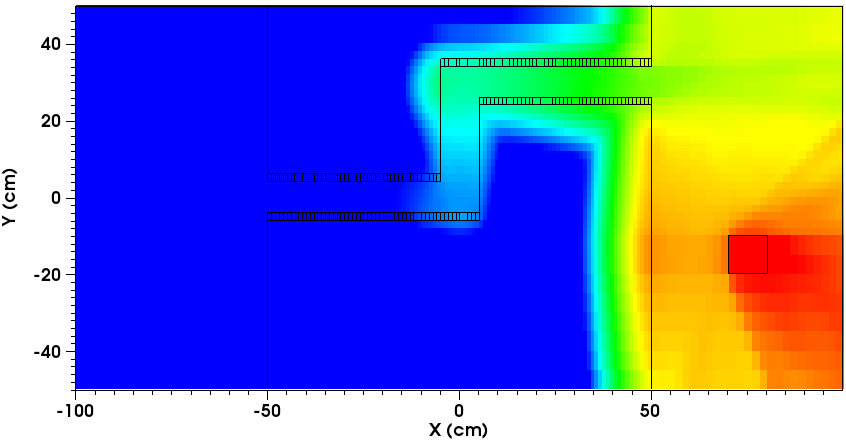
\includegraphics[height=1in,clip]{maze2_myflux_group26_adjusted_cropped.png}
%  		%\caption{Adjoint flux used by CADIS-$\Omega$}
%  	\end{center}
%  	\end{figure}
%  	\end{column}
%	\end{columns}
%	\vspace*{1 em}
%	.... shows that the method does incorporate problem physics differently
%  
%	
%\end{frame}
%
%%% --------------------------------------------------------------
%%
%\begin{frame}[fragile]
%  \frametitle{Response in detector}
%  
%\begin{columns}
%  \begin{column}{0.45\textwidth}
%  Adjusted CADIS has:
%  \begin{itemize}
%    \item Relatively uniform uncertainty distribution
%    \item Raster runtimes than CADIS
%    \item Better overall results than analog
%  \end{itemize}
%  \begin{tabular}{|l|c c|}
%  \hline
%      Run Type & FOM$_{MC}$ & FOM$_{adj}$ \\  
%      \hline
%      Analog & 493 & 493 \\
%      CADIS  & 8   &   7 \\
%      CADIS-$\Omega$ & 466 & 354 \\
%      \hline
%  \end{tabular}
%  \end{column}
%  \begin{column}{0.55\textwidth}
%  	\begin{figure}
%  	\begin{center}
%  		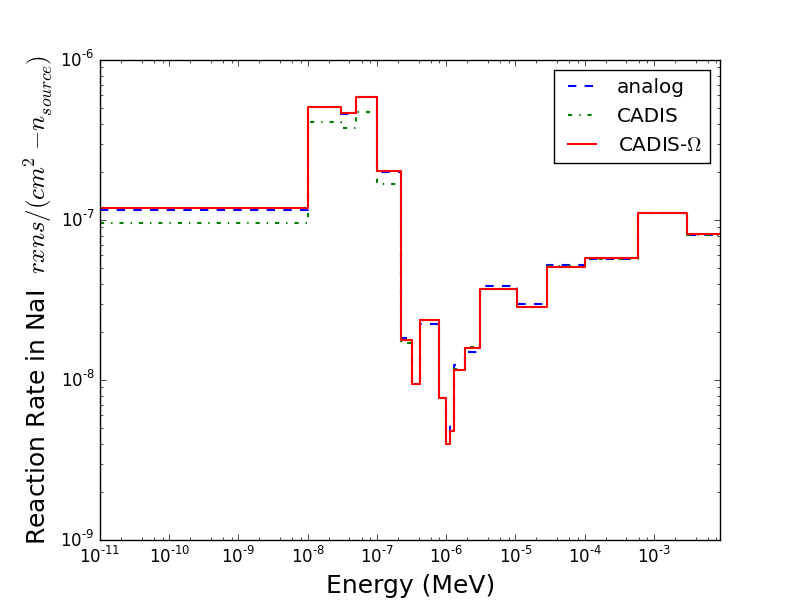
\includegraphics[height=1.3in,clip]{response.png}
%		%\caption{Response for maze 2}
%	\end{center}
%  	\end{figure}
%  	  \begin{figure}
%  	\begin{center}
%  		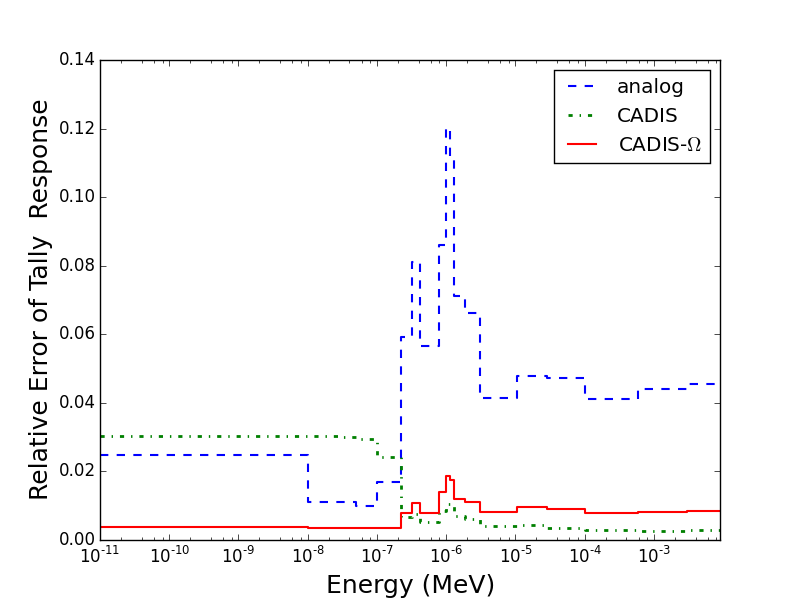
\includegraphics[height=1.3in,clip]{response_RE.png}
%		%\caption{Relative errors for response function}
%		% point out that while the FOM is better for analog, it has high RE in regions, so overall it performs poorer
%	\end{center}
%  	\end{figure}
%  \end{column}
%\end{columns}
%	
%\end{frame}

%% --------------------------------------------------------------
%% --------------------------------------------------------------
%\section{\scshape Continuing Work}
\begin{frame}[fragile]

  \frametitle{Characterization Tests}
   Quantify method's effectiveness for problems with different degrees of anisotropy: \\
   \vspace*{1 em}
    Spatial streaming; \hspace*{2 em} Labyrinth variants;\\
    Spherical boat; \hspace*{4.25 em} Energy streaming
    \vspace{1 em}
    
%    \begin{columns}
%    \begin{column}{0.45\textwidth}
%    \textbf{Deterministic}
%    \begin{itemize}
%    \item Energy groups 
%    \item Quadrature order
%    \item Quadrature type
%    \item Spatial discretization
%    \end{itemize}
%    \end{column}
%    
%    \begin{column}{0.55\textwidth}
%    \textbf{Monte Carlo}
%    \begin{itemize}
%    \item Tally spatial resolution (FW CADIS only)
%    \item Tally energy resolution 
%    \end{itemize}
%    \end{column}
%  \end{columns}

\end{frame}

%% --------------------------------------------------------------

\begin{frame}[fragile]

  \frametitle{Impact Tests}
  
    \begin{columns}
    \begin{column}{0.55\textwidth}
    Real system tests will show the ability of the method to improve MC for applications of interest\\
    \vspace*{1em}
    We are starting with a full storage cask with highly-detailed information
    \end{column}    
    \begin{column}{0.45\textwidth}
  \begin{center}
  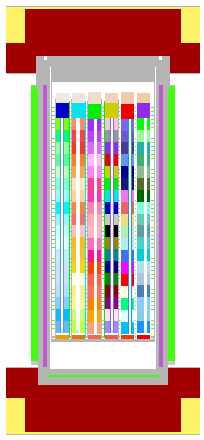
\includegraphics[height=2.5in,clip]{Transfer_Side_profile}  
  \end{center}
    \end{column}
  \end{columns}   

\end{frame}

% --------------------------------------------------------------
% --------------------------------------------------------------


%% --------------------------------------------------------------
%% --------------------------------------------------------------
\section{\scshape LDO Method}
\begin{frame}[fragile]

  \frametitle{Lagrange Discrete Ordinates (LDO) \cite{Ahrens2015}}

   We're also looking at an entirely different approach.    
\pause
\begin{itemize}
\item{Formally the same as the classical $S_N$ equations}
	\begin{itemize}
	\pause
	\item{The difference lies in how the scattering source is calculated and in the representation of the angular flux}
	\pause
	\item{\textbf{No need to evaluate spherical harmonic moments of angular flux}}
	\end{itemize}
\pause
\item{Increasing the angular resolution of the LDO equations brings ability to mitigate ray effects}
%	\begin{itemize}
%	\pause
%	\item{Positive-weight quadrature sets on which LDO equations are based can integrate spherical harmonics from degree 0 to degree 165}
%	\pause
%	\item{For a fixed maximum degree of integration $N$, the corresponding number of quadrature points (ordinates) is $(N+1)^2$}
%	\end{itemize}
\pause
\item{\textbf{LDO equations naturally allow angular flux to be evaluated in directions other than those found in the quadrature set}}
	\begin{itemize}
	\pause
	\item{Solution of the LDO equations has interpolatory structure in angle}
	\pause
	\item{Opens the door to using angular biasing schemes for hybrid Monte Carlo calculations}
	\end{itemize}
\end{itemize}

\end{frame}

% --------------------------------------------------------------
%\begin{frame}{Lagrange Discrete Ordinates (LDO) Equations}
%\begin{multline}
%\vOmega_i\cdot\nabla\psi_i^g(\vecr) + \Sigma_t^g(\vecr)\psi_i^g(\vecr) \\ \qquad= 
%\sum_{g'=1}^{G}\sum_{j=1}^{\dn}\sum_{i'=1}^{\dn}\langle L_{i'},L_j\rangle\Sigma_{s,N}^{g'\rightarrow g}(\vecr,\vOmega_i\cdot\vOmega_j)\psi_{i'}^{g'}(\vecr) + S^g(\vecr,\vOmega_i);~ \\
%i =1,2,\ldots,\dn;~g=1,2,\ldots,G
%\end{multline}
%These are the multigroup LDO equations, which are formally the same as the classical $S_N$ equations. The difference lies in how the scattering source is calculated and in the representation of the angular flux.
%\end{frame}


\begin{frame}{Derivation of the LDO Equations}
Start with the TE:
\begin{multline}
\vOmega\cdot  \nabla \psi(\vecr,E,\vOmega) + \Sigma_t(\vecr,E)\psi(\vecr,E,\vOmega) = S(\vecr, E, \vOmega) 
\\ +
\int_0^{\infty}\int_{\maths}\Sigma_s(\vecr, E'\rightarrow E,\vOmega'\cdot\vOmega)
\psi(\vecr,E',\vOmega')d\vOmega'dE'
\end{multline}
\begin{itemize}
\pause
\item{Define approximation $\psi_N(\vecr,E,\vOmega) = \sum_{i=1}^{\dn}\psi_i(\vecr,E)L_i(\vOmega)$ and substitute it into the TE}
\pause
\item{$\psi_i(\vecr,E)$ are flux coefficients, $L_i(\vOmega)$ is the $i^{th}$ Lagrange element}
\pause
\item{$\dn\equiv \dim\hn = (N+1)^2$;
 
 $\hn = \text{span}\{Y^m_n: |m| \leq n, 0 \leq n \leq N\}$}
\end{itemize}
\end{frame}

%\begin{frame}{Lagrange Functions \cite{sph}}
%Defined generally as:
%\begin{equation}
%L_i(\vOmega) =
%\frac{
%\det
%\begin{bmatrix}
%\ell_1(\vOmega_1)&\cdots&\ell_n(\vOmega_1) &\cdots& \ell_P(\vOmega_1) \\
%\vdots & \ddots & \vdots & \ddots & \vdots \\
%\ell_1(\vOmega_{i-1}) & \cdots &\ell_n(\vOmega_{i-1}) & \cdots & \ell_P(\vOmega_{i-1}) \\
%\ell_1(\vOmega) & \cdots & \ell_n(\vOmega) & \cdots & \ell_P(\vOmega) \\
%\ell_1(\vOmega_{i+1}) & \cdots & \ell_n(\vOmega_{i+1}) & \cdots & \ell_P(\vOmega_{i+1}) \\
% \vdots & \ddots & \vdots & \ddots & \vdots \\
%\ell_1(\vOmega_P) & \cdots & \ell_n(\vOmega_P) & \cdots & \ell_P(\vOmega_P)
% \end{bmatrix} 
%}
%{
%\det
%\begin{bmatrix}
%\ell_1(\vOmega_1)&\cdots&\ell_n(\vOmega_1) &\cdots& \ell_P(\vOmega_1) \\
% \vdots & \ddots & \vdots & \ddots & \vdots \\
%\ell_1(\vOmega_i)&\cdots&\ell_n(\vOmega_i) &\cdots& \ell_P(\vOmega_i) \\
% \vdots & \ddots & \vdots & \ddots & \vdots \\
%\ell_1(\vOmega_P)&\cdots&\ell_n(\vOmega_P) &\cdots& \ell_P(\vOmega_P)
% \end{bmatrix} 
%}
%\end{equation}
%Here, $\{\vOmega_1,\ldots,\vOmega_P\}$ varies over $\maths$ and $\{\ell_1,\ldots,\ell_P\}$ are basis functions for the space of polynomials of degree $\leq P$.
%% pgs 190 and 133 of springer book, maybe ask
%% look up basis functions and know how to talk about them!
%% what can they be, what do we usually choose for them, etc.
%\end{frame}

\begin{frame}{Lagrange Functions (cont'd.)}

The $L_{i}(\vOmega)$ satisfy:
\begin{equation}
L_i(\vOmega_j) = \delta_{i,j};\quad i,j = 1,2,\ldots,P;\quad P = \dn
\end{equation}
\pause
Interpolatory points allow definition of a quadrature for $f \in \hn$% = \text{span}\{Y^m_n: |m| \leq n, 0 \leq n \leq N\};\ \dim\hn = (N+1)^2 \equiv \dn$:
\begin{equation}
\int_{\maths}f(\vOmega)d\vOmega = \int_{\maths}\sum_{i=1}^{\dn} f_i L_i(\vOmega)d\vOmega 
= \sum_{i=1}^{\dn}\int_{\maths}L_i(\vOmega)d\vOmega f_i = \sum_{i=1}^{\dn} w_i f_i
\end{equation}
\pause
Quadrature weights:
\begin{equation}
w_i = \int_{\maths}L_{i}(\vOmega)d\vOmega = \sum_{j=1}^{\dn}\lij
\end{equation}
%Here, $\langle f,g\rangle$ is the inner product $\int_{\maths}f(\vOmega)g(\vOmega)d\vOmega$.
\end{frame}

\begin{frame}[label=group_disc]{Derivation of the LDO Equations (cont'd.)}
%Define the residual:
%\begin{multline}
%r_N(\vecr,E,\vOmega) \equiv \vOmega\cdot\nabla\psi_N(\vecr,E,\vOmega) + \sigt(\vecr,E)\psi_N(\vecr,E,\vOmega) \\
%- \int_{0}^{\infty}\int_{\maths}\sigs(\vecr,E'\rightarrow E, \vOmega'\cdot\vOmega)\psi_N(\vecr,E',\vOmega')d\vOmega'dE' - S(\vecr,E,\vOmega)
%\end{multline}
%\pause
\begin{itemize}
\item Discretize the energy variable with a standard multigroup approach
%\begin{multline}
%r_N^g = \vOmega\cdot\sum_{i=1}^{\dn}\left[\nabla\psi_i^g(\vecr)\right]L_i(\vOmega) + \Sigma_t^g(\vecr)\sum_{i=1}^{\dn}\psi_i^g(\vecr)L_i(\vOmega) \\
%- \sum_{g'=1}^G\sum_{i'=1}^{\dn} \psi_{i'}^{g'}(\vecr)\int_{\maths}\Sigma_{s}^{g'\rightarrow g}(\vecr,\vOmega'\cdot\vOmega)L_{i'}(\vOmega')d\vOmega'
%- S^g(\vecr,\vOmega); \\ g=1,2,\ldots,G
%\end{multline}
%\end{frame}
%\
\pause
%\begin{frame}[label=ldo-fin]{Derivation of the LDO Equations (cont'd.)}
\item Analytically evaluate the scattering cross section and substitute it in%into the residual
\end{itemize}
%\begin{multline}
%r_N^g = \vOmega\cdot\sum_{i=1}^{\dn}\left[\nabla\psi_i^g(\vecr)\right]L_i(\vOmega) + \Sigma_t^g(\vecr)\sum_{i=1}^{\dn}\psi_i^g(\vecr)L_i(\vOmega) \\
%- \sum_{g'=1}^{G}\sum_{j=1}^{\dn}\sum_{i'=1}^{\dn}\langle L_{i'},L_j\rangle\Sigma_{s,N}^{g'\rightarrow g}(\vecr,\vOmega_j\cdot\vOmega)\psi_{i'}^{g'}(\vecr) - S^g(\vecr,\vOmega)
%\end{multline}
\pause
We invoke a collocation procedure that requires the residual to be zero at the points 
$\{\vOmega_i\}_{i=1}^{\dn}$, leading to the $G\times\dn$ equations:
\begin{multline}
\vOmega_i\cdot\nabla\psi_i^g(\vecr) + \Sigma_t^g(\vecr)\psi_i^g(\vecr) \\ \qquad= 
\sum_{g'=1}^{G}\sum_{j=1}^{\dn}\sum_{i'=1}^{\dn}\langle L_{i'},L_j\rangle\Sigma_{s,N}^{g'\rightarrow g}(\vecr,\vOmega_i\cdot\vOmega_j)\psi_{i'}^{g'}(\vecr) + S^g(\vecr,\vOmega_i)%;~ \\
%i =1,2,\ldots,\dn;~g=1,2,\ldots,G
\end{multline}
These are the new multigroup LDO equations.
\end{frame}


% --------------------------------------------------------------
% --------------------------------------------------------------
\section*{}
\begin{frame}[fragile]
  \frametitle{Summary}
  \begin{itemize}
  \item Need for methods
  \item CADIS-$\vOmega$...
  \item LDO
  \end{itemize}
\end{frame}


% --------------------------------------------------------------
% --------------------------------------------------------------
\section*{}
\begin{frame}[fragile]
  \frametitle{Questions?}
  \begin{center}
  \includegraphics[height=3in,clip]{../questions-comic}  
  \end{center}
  
\end{frame}

% --------------------------------------------------------------
\begin{frame}[allowframebreaks]{References}
	\bibliographystyle{unsrt}
	\bibliography{2017-03-mpact}
\end{frame}

\end{document}
